\subsection{Mainboard PCB}
\textit{(pro)} Um die Elektronik Komponenten auf übersichtliche und zuverlässige Weise miteinander zu verknüpfen wurde ein 2-Lagiges PCB designt, welches als Prototyp an der HSLU T\&A gefertig werden kann. Durch ein PCB wird der Verdrahtungsaufwand zwischen den Komponenten auf ein Minimum reduziert. In den folgenden Unterkapiteln wird das Schema, die verwendeten Elektronik Bauteile und das Layout des Mainboard PCBs erklärt.
\subsubsection{FRDM-KL25Z Header}
Das Mainboard PCB verbindet sämtliche Elektronik Komponenten miteinander. Das Herzstück bildet dabei das Mikrocontroller Board FRDM-KL25Z von NXP, welches über Stiftleisten auf das Mainboard aufgesteckt wird. Es verfügt über einen 32-bit ARM Cortex M0+ Mikrocontroller mit einer Taktrate von 48MHz, 128KB Flash und 16KB RAM. In der folgenden Tabelle werden die Signale welche vom FRDM-Board zur Verfügung gestellt werden aufgeführt. Die Spalten der Tabelle sind wie folgt zu lesen: \textbf{CON} ist der Stecker mit der jeweiligen Pin Nummer, \textbf{Port} beschreibt den Pin des uC, \textbf{Mapping} gibt an für was der Port des uC verwendet wird und \textbf{Funktion} beschreibt die Verwendung des uC Pins auf dem Mainboard PCB.

% Table generated by Excel2LaTeX from sheet 'FRDM-KL25z Port Mapping'
\begin{table}[H]
	\scriptsize
	\centering
	\caption{FRDM-KL25Z Port Mapping}
	\begin{tabular}{|r|r|r|r|l|l|r|l|}
		\hline
		\multicolumn{1}{|l|}{\textbf{CON}} & \multicolumn{1}{l|}{\textbf{Port}} & \multicolumn{1}{l|}{\textbf{Mapping}} & \multicolumn{1}{l|}{\textbf{Funktion}} & \textbf{CON} & \textbf{Port} & \multicolumn{1}{l|}{\textbf{Mapping}} & \textbf{Funktion} \\
		\hline
		\multicolumn{1}{|l|}{J1 01} & \multicolumn{1}{l|}{PTC7} &       & \multicolumn{1}{l|}{NC} & J2 01 & PTC12 & \multicolumn{1}{l|}{Digital In} & BTN\_tiefer \\
		\hline
		\multicolumn{1}{|l|}{J1 02} & \multicolumn{1}{l|}{PTA1 } & \multicolumn{1}{l|}{UART0\_RX} & \multicolumn{1}{l|}{Bluetooth RX} & J2 02 & PTA13  & \multicolumn{1}{l|}{FTM1\_CH1} & Vibramotors 1 \\
		\hline
		\multicolumn{1}{|l|}{J1 03} & \multicolumn{1}{l|}{PTC0} & \multicolumn{1}{l|}{ADC0\_SE14} & \multicolumn{1}{l|}{IR-Sensor} & J2 03 & PTC13 & \multicolumn{1}{l|}{Digital In} & BTN\_höher \\
		\hline
		\multicolumn{1}{|l|}{J1 04} & \multicolumn{1}{l|}{PTA2 } & \multicolumn{1}{l|}{UART0\_TX} & \multicolumn{1}{l|}{Bluetooth TX} & J2 04 & PTD5  & \multicolumn{1}{l|}{Digital Out} & CSN nRF24L01+ \\
		\hline
		\multicolumn{1}{|l|}{J1 05} & \multicolumn{1}{l|}{PTC3} &       & \multicolumn{1}{l|}{NC} & J2 05 & PTC16 & \multicolumn{1}{l|}{Digital In} & BTN Vereinzeln \\
		\hline
		\multicolumn{1}{|l|}{J1 06} & \multicolumn{1}{l|}{PTD4 } & \multicolumn{1}{l|}{Digital Out} & \multicolumn{1}{l|}{DC\_OK} & J2 06 & PTD0  & \multicolumn{1}{l|}{Digital Out} & CE nRF24L01+ \\
		\hline
		\multicolumn{1}{|l|}{J1 07} & \multicolumn{1}{l|}{PTC4} &       & \multicolumn{1}{l|}{NC} & J2 07 & PTC17 & \multicolumn{1}{l|}{Digital In} & BTN Spindel runter \\
		\hline
		\multicolumn{1}{|l|}{J1 08} & \multicolumn{1}{l|}{PTA12 } & \multicolumn{1}{l|}{FTM1\_CH0} & \multicolumn{1}{l|}{Vibramotors 2} & J2 08 & PTD2  & \multicolumn{1}{l|}{SPI0\_MOSI} & nRF24L01+ \\
		\hline
		\multicolumn{1}{|l|}{J1 09} & \multicolumn{1}{l|}{PTC5} &       & \multicolumn{1}{l|}{NC} & J2 09 & PTA16  & \multicolumn{1}{l|}{Digital In} & BTN Spindel hoch \\
		\hline
		\multicolumn{1}{|l|}{J1 10} & \multicolumn{1}{l|}{PTA4 } & \multicolumn{1}{l|}{Digital Out} & \multicolumn{1}{l|}{Servo enable} & J2 10 & PTD3  & \multicolumn{1}{l|}{SPI0\_MISO} & nRF24L01+ \\
		\hline
		\multicolumn{1}{|l|}{J1 11} & \multicolumn{1}{l|}{PTC6} &       & \multicolumn{1}{l|}{NC} & J2 11 & PTA17  &       & NC \\
		\hline
		\multicolumn{1}{|l|}{J1 12} & \multicolumn{1}{l|}{PTA5 } & \multicolumn{1}{l|}{FTM0\_CH2} & \multicolumn{1}{l|}{ION enable} & J2 12 & PTD1  & \multicolumn{1}{l|}{SPI0\_SCK} & nRF24L01+ \\
		\hline
		\multicolumn{1}{|l|}{J1 13} & \multicolumn{1}{l|}{PTC10} & \multicolumn{1}{l|}{I2C1\_SDA} & \multicolumn{1}{l|}{LED Driver} & J2 13 & PTE31 & \multicolumn{1}{l|}{FTM0\_CH4} & Servo 3 \\
		\hline
		\multicolumn{1}{|l|}{J1 14} & \multicolumn{1}{l|}{PTC8 } & \multicolumn{1}{l|}{Digital Out} & \multicolumn{1}{l|}{Stop\_In} & J2 17 & PTD6  &       & NC \\
		\hline
		\multicolumn{1}{|l|}{J1 15} & \multicolumn{1}{l|}{PTC11} & \multicolumn{1}{l|}{I2C1\_SCL } & \multicolumn{1}{l|}{LED Driver} & J2 18 & PTE1  & \multicolumn{1}{l|}{UART1\_RX} & TMCM-1630 TX \\
		\hline
		\multicolumn{1}{|l|}{J1 16} & \multicolumn{1}{l|}{PTC9 } & \multicolumn{1}{l|}{Digital Out} & \multicolumn{1}{l|}{IRQ nRF24L01+} & J2 19 & PTD7  &       & NC \\
		\hline
		\multicolumn{1}{|l|}{J10 01} & \multicolumn{1}{l|}{PTE20} & \multicolumn{1}{l|}{ADC0\_SE0} & \multicolumn{1}{l|}{IR Sensor 2} & J2 20 & PTE0  & \multicolumn{1}{l|}{UART1\_TX } & TMCM-1630 RX \\
		\hline
		\multicolumn{1}{|l|}{J10 02} & \multicolumn{1}{l|}{PTB0 } & \multicolumn{1}{l|}{ADC0\_SE8} & \multicolumn{1}{l|}{IR Sensor 1} & J9 01 & PTB8  & \multicolumn{1}{l|}{Digital In} & BTN\_AUTO \\
		\hline
		\multicolumn{1}{|l|}{J10 03} & \multicolumn{1}{l|}{PTE21} &       & \multicolumn{1}{l|}{NC} & J9 03 & PTB9  & \multicolumn{1}{l|}{Digital In} & BTN\_14cm \\
		\hline
		\multicolumn{1}{|l|}{J10 04} & \multicolumn{1}{l|}{PTB1 } &       & \multicolumn{1}{l|}{Spare GPIO} & J9 05 & PTB10 & \multicolumn{1}{l|}{Digital In} & BTN\_13cm \\
		\hline
		\multicolumn{1}{|l|}{J10 05} & \multicolumn{1}{l|}{PTE22 } & \multicolumn{1}{l|}{UART2\_TX} & \multicolumn{1}{l|}{RoboClaw RX} & J9 07 & PTB11 & \multicolumn{1}{l|}{Digital In} & BTN\_12cm \\
		\hline
		\multicolumn{1}{|l|}{J10 06} & \multicolumn{1}{l|}{PTB2 } &       & \multicolumn{1}{l|}{Spare GPIO} & J9 09 & PTE2  & \multicolumn{1}{l|}{Digital In} & BTN\_11cm \\
		\hline
		\multicolumn{1}{|l|}{J10 07} & \multicolumn{1}{l|}{PTE23} & \multicolumn{1}{l|}{UART2\_RX} & \multicolumn{1}{l|}{RoboClaw TX} & J9 10 & P5V\_USB &       & NC \\
		\hline
		\multicolumn{1}{|l|}{J10 08} & \multicolumn{1}{l|}{PTB3 } &       & \multicolumn{1}{l|}{Spare GPIO} & J9 11 & PTE3  & \multicolumn{1}{l|}{Digital In} & BTN\_9cm \\
		\hline
		\multicolumn{1}{|l|}{J10 09} & \multicolumn{1}{l|}{PTE29} & \multicolumn{1}{l|}{FTM0\_CH2} & \multicolumn{1}{l|}{Servo 1} & J9 12 & GND   & \multicolumn{1}{l|}{GND} & GND \\
		\hline
		\multicolumn{1}{|l|}{J10 10} & \multicolumn{1}{l|}{PTC2} &       & \multicolumn{1}{l|}{Spare GPIO} & J9 13 & PTE4  &       & NC \\
		\hline
		\multicolumn{1}{|l|}{J10 11} & \multicolumn{1}{l|}{PTE30} & \multicolumn{1}{l|}{FTM0\_CH3} & \multicolumn{1}{l|}{Servo 2} & J9 14 & GND   & \multicolumn{1}{l|}{GND} & GND \\
		\hline
		\multicolumn{1}{|l|}{J10 12} & \multicolumn{1}{l|}{PTC1} &       & \multicolumn{1}{l|}{Spare GPIO} & J9 15 & PTE5  &       & Spare GPIO \\
		\hline
		&       &       &       & J9 16 & P5-9V\_VIN &       & 5VCC \\
		\hline
	\end{tabular}%
	\label{tab:FRDM_Port_Mapping}%
\end{table}%

Beim Design des Mainboard PCBs wurde darauf geachtet, dass möglichst viele GPIO Pins des FRDM-Boards genutzt werden. Deshalb wurde zusätzlich zu den in Abbildung \ref{fig:Blockschaltbild_Komponenten} aufgeführten Peripherien, ein Servo Interface mit drei Servo Anschlüssen und eine Buchsenleiste mit zusätzlichen GPIOs vorgesehen.

\subsubsection{Anschlüsse}
Die im vorhergehenden Kapitel beschriebenen Signale werden über Steckverbindungen auf das Mainboard geführt. Die Steckverbindungen sind in Abb. \ref{fig:Mainboard_3D} mit einer jeweiligen Beschriftungen illustriert. Die Anschlüsse welche nicht beschriftet sind gehören zum HMI und werden im Kapitel \ref{sec:Mainboard_HMI_Interface} behandelt. Für Signalleitungen und Speiseleitungen bis 2A werden JST Stecker der Serie PH mit 2, 3, 4 und 6 Pol verwendet. Diese haben ein schmales Rastermass von 2mm und eignen sich daher gut für kompakte PCB Anwendungen. Die 12V Speisung und das ION Motion Interface werden über 90° Phoenix Stiftleisten der Serie MSTBA geführt. Diese Stecker sind mit einem Nennstrom von 10A gemäss UL Zertifizierung zugelassen.

\begin{figure}[H]
	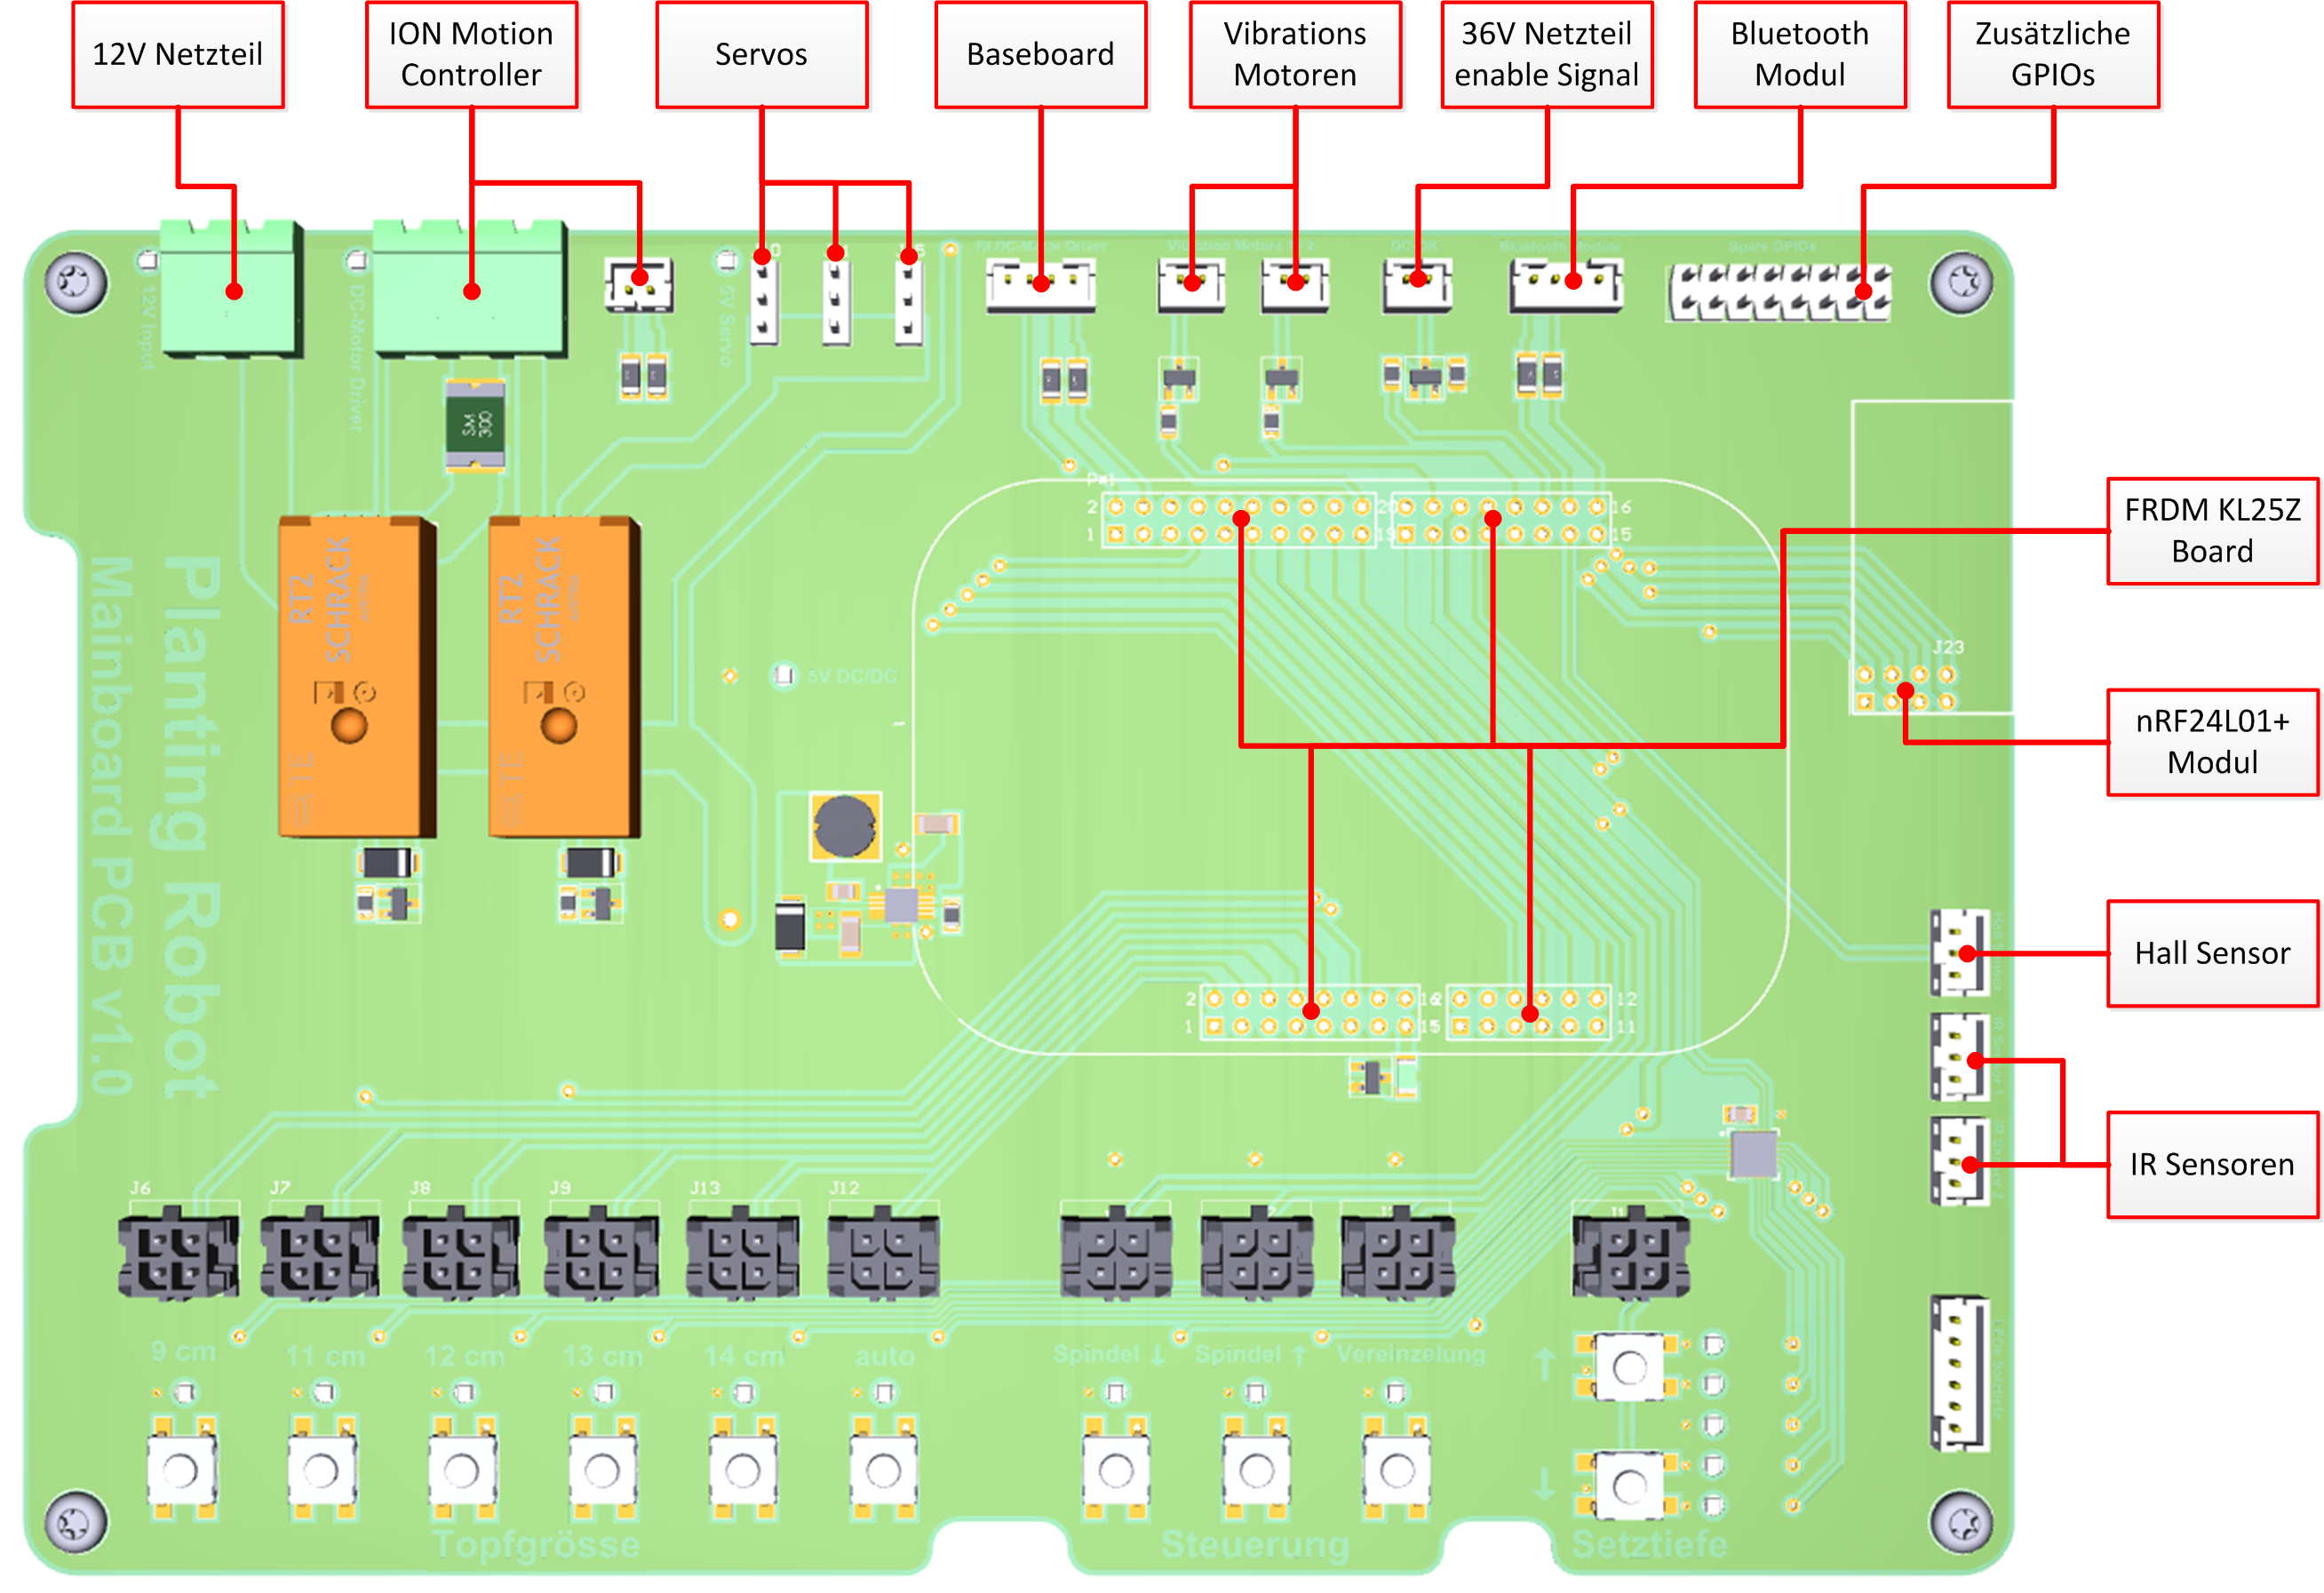
\includegraphics[width=1\textwidth]{Illustrationen/6-Umsetzung/Mainboard_PCB_Anschluesse.jpg}
	\caption{Mainboard PCB, Anschlüsse}
	\label{fig:Mainboard_3D}
\end{figure}

Um allfällig zusätzliche Peripherie mit dem FRDM-Board verbinden zu können, ist eine zweireihige 16P Stiftleiste mit 6 GPIO Ports, einer I$^{2}$C Schnittstelle, einem 5V und 12V Spannungspin vorgesehen. Des weiteren werden können das FRDM-Board und das nRF24L01+ Modul über Stiftleisten auf das Mainboard PCB gesteckt werden.

\subsubsection{Power Supply}
In Abb. \ref{fig:Schema_Mainboard_PowerSupply_1} sowie \ref{fig:Schema_Mainboard_PowerSupply_2} ist der Power Supply Teil des Schemas vom Mainboard PCB abgebildet. Das Mainboard wird über das selbe 12V Netzteil mit Strom versorgt wie der ION Motion Motorcontroller. Um die Stromversorgung des Motorcontrollers schalten zu können wird diese über das Mainboard geführt. Auf dem Mainboard PCB befindet sich dann das Relais U3, welches vom uC gesteuert wird. Ebenfalls schaltbar ist die 5V Speisung des Servo Interfaces über das Relais U2. Dieses Spannungspotential wird vom ION Motion Controller abgegriffen. Dieser Verfügt über einen 5V Spannungswandler welcher bis zu 3A liefern kann. 

\begin{figure}[H]
	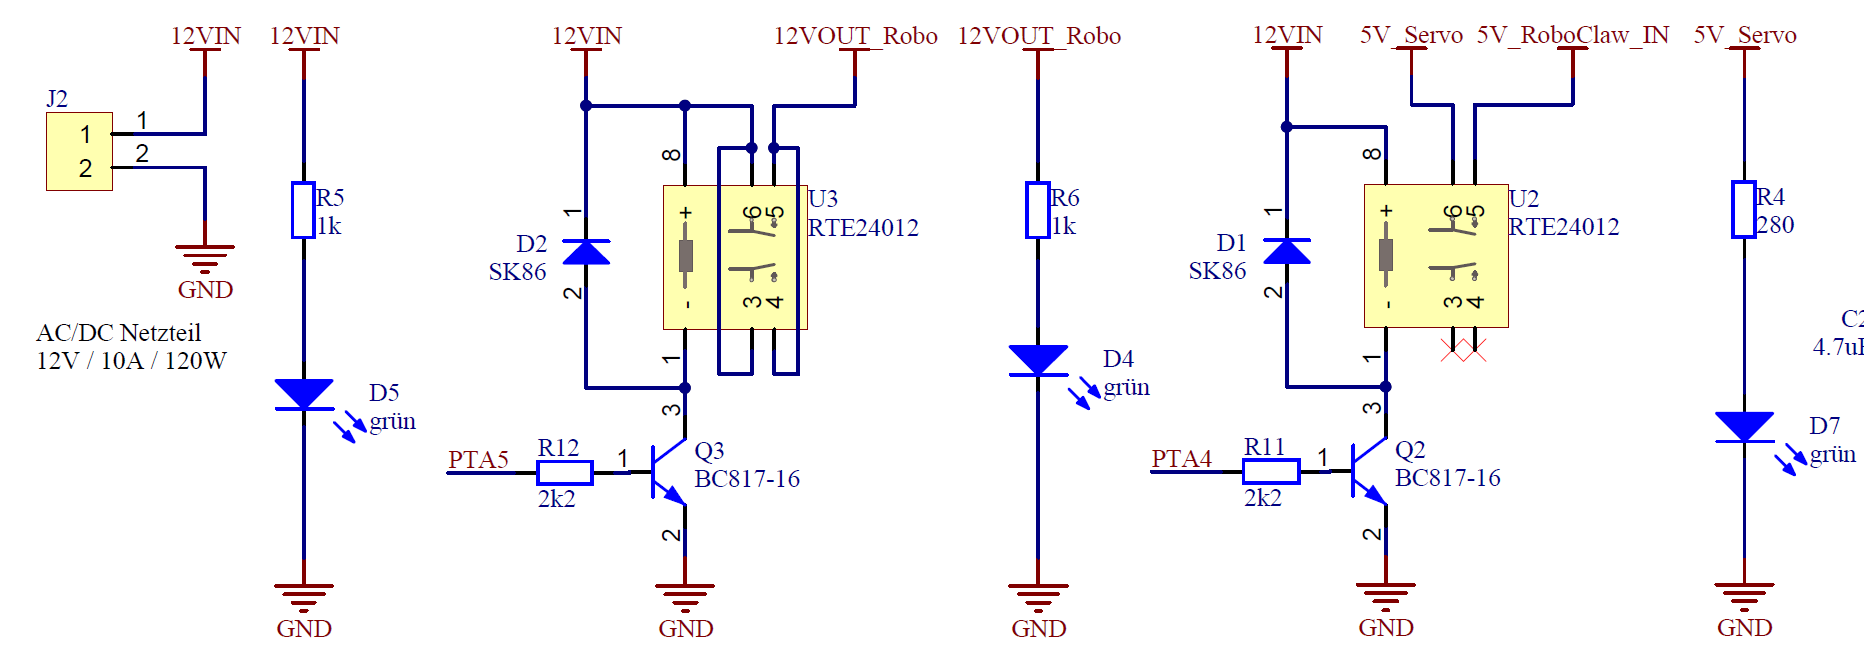
\includegraphics[width=0.8\textwidth]{Illustrationen/6-Umsetzung/Schema_Mainboard_PowerSupply_1.png}
	\caption{Schema Mainboard PCB, Power Supply Relais}
	\label{fig:Schema_Mainboard_PowerSupply_1}
\end{figure}

Die Speisung für den BLDC Motor kann über das DC$\_$OK Signal des 36V Netzteils geschalten werden. Das DC-OK Signal ist ein TTL Signal und wird deshalb über den Transistor Q1 vom uC geschaltet.

\begin{figure}[H]
	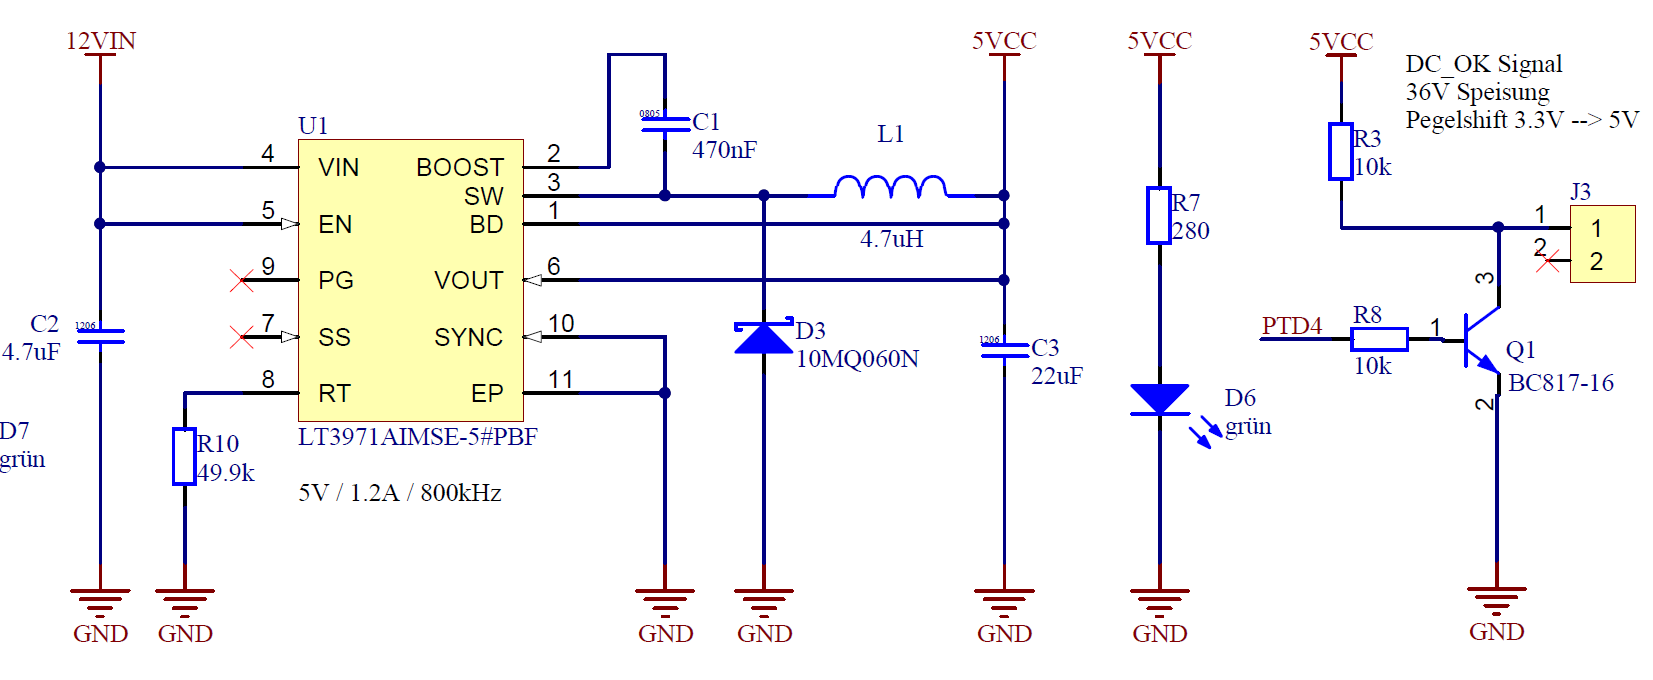
\includegraphics[width=0.8\textwidth]{Illustrationen/6-Umsetzung/Schema_Mainboard_PowerSupply_2.png}
	\caption{Schema Mainboard PCB, Power Supply DC/DC-Wandler}
	\label{fig:Schema_Mainboard_PowerSupply_2}
\end{figure}


Die Spannungsversorgung für das FRDM-Board, den LED Treiber, die Sensoren und die Vibrationsmotoren wird durch den DC/DC-Festspannungsregler LT3971 bereit gestellt. In der folgenden Tabelle sind die wichtigsten Daten des Buck Reglers ausgeführt:

% Table generated by Excel2LaTeX from sheet 'LT3971 Datasheet'
\begin{table}[htbp]
	\small
	\centering
	\caption{LT3971 Überblick Daten \protect\cite{LT3971_Datasheet}}
	\begin{tabular}{|l|ccc|r|}
		\hline
		\textbf{Parameter} & \multicolumn{1}{l}{\textbf{MIN}} & \multicolumn{1}{l}{\textbf{TYP}} & \multicolumn{1}{l}{\textbf{MAX}} & \textbf{Einheit} \\
		\hline
		Eingangsspannung &       &       & 38    & V \\
		\hline
		Ausgangsspannung & 4.93  & 5     & 5.07  & V \\
		\hline
		Ausgangsstrom &       &       & 1.2   & A \\
		\hline
		Schaltfrequenz & 0.2   &       & 2     & MHz \\
		\hline
		Wirkungsgrad &       & 85    &       & \% \\
		\hline
	\end{tabular}%
	\label{tab:LT3971_Datasheet}%
\end{table}%

Bei einem getakteten Spannungswandler sollte das Layout gemäss den Design Richtlinien des Herstellers erstellt werden. Dadurch wird garantiert, dass die Funktionalität und die EMV Eigenschaften der Schaltung auf einem hohen Niveau sind. Die Bauteilwerte der Schaltung wurden der typical application des Datenblatts entnommen. Der Buck Regler wird demanch mit einer Schaltfrequenz von 800kHz betrieben. In Abb. \ref{fig:LT2971_Layout} ist links der Auszug aus dem Datenblatt und rechts das Layout auf dem Mainboard PCB abgebildet. Die Bauteilbezeichnungen korrespondieren dabei nicht miteinander.

\begin{figure}[H]
	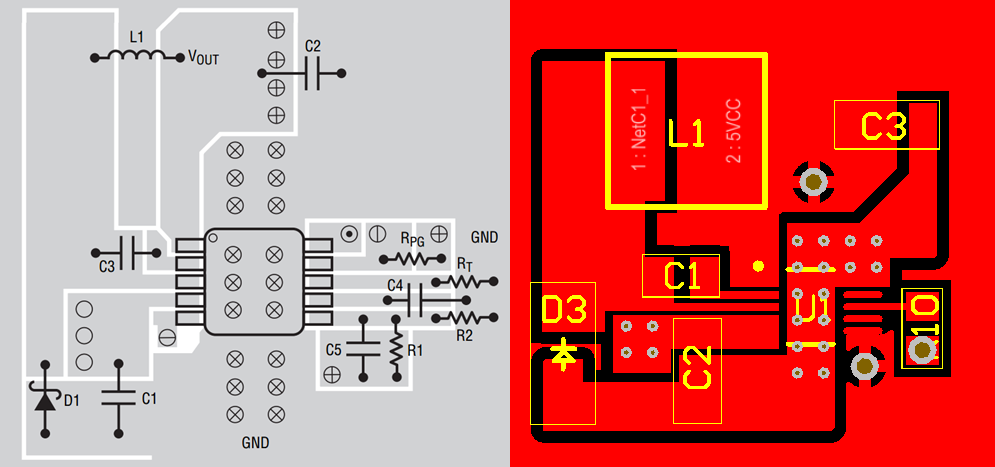
\includegraphics[width=0.8\textwidth]{Illustrationen/6-Umsetzung/LT3971_Layout.png}
	\caption{Layout LT3971: Datenblatt \protect\cite{LT3971_Datasheet}, Mainboard PCB}
	\label{fig:LT2971_Layout}
\end{figure}

\subsubsection{HMI Interface} \label{sec:Mainboard_HMI_Interface}
Das HMI bildet die Schnittstelle zwischen Operator und Planting Robot. Der Planting Robot soll so einfach wie möglich zu bedienen sein. Auf ein Touchscreen Interface oder Displays mit Menüführung durch Taster wird daher bewusst verzichtet. Stattdessen werden Taster mit blau, grün und weisser LED-Ring Beleuchtung (siehe Abb. \ref{fig:Taster_LED-Ring}) verwendet. Die Funktionen des Planting Robots werden dabei durch korrespondierende Taster realisiert. Die Funktionen des HMI werden in Kapitel \ref{sec:HMI} erklärt.
\begin{figure}[H]
	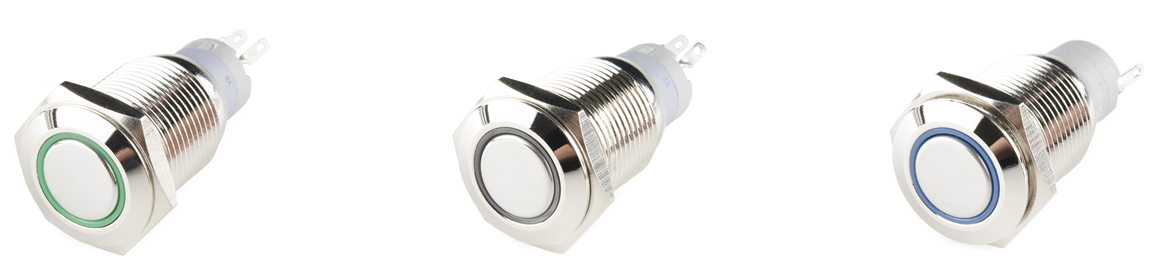
\includegraphics[width=0.7\textwidth]{Illustrationen/6-Umsetzung/HMI_LED_Taster.png}
	\caption{HMI Taster mit LED Ring \protect\cite{HMI_Taster}}
	\label{fig:Taster_LED-Ring}
\end{figure}

In Summe werden für das HMI 11 Taster und 14 LEDs angesteuert. Gemäss Tabelle \ref{tab:FRDM_Port_Mapping} sind zu wenig freie GPIO Ports Verfügbar um das HMI vollständig an Digital I/O Pins des FRDM-Boards anzuschliessen. Um die Anzahl benötigter GPIOs zu reduzieren können folgende Beschaltungen verwendet werden:
\begin{itemize}
	\item Testerauswertung über eine Keyboard Matrix
	\item LED Ansteuerung durch einen LED Treiber
\end{itemize}

Eine Keyboard Matrix kann über ein entsprechendes IC wie z.B. den LM8330 von TI realisiert werden. Dieses IC wird an den I$^2$C Bus angeschlossen und übernimmt die Matrizenauswertung inklusive entprellen der Taster. Der LM8330 ist allerdings nur im DSBGA Package (siehe Abb. \ref{fig:DSBGA_Package}), in der Grösse 2mm x 2mm, erhältlich. Dieses Package ist im Leiterplatten Prototypenbau nicht verwendbar, da es nicht von Hand bestückt werden kann.\newline

\begin{figure}[H]
	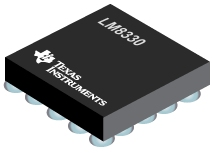
\includegraphics[width=0.27\textwidth]{Illustrationen/6-Umsetzung/DSBGA_Package.png}
	\caption{LM8330 DSBGA Package \protect\cite{DSBGA_Package}}
	\label{fig:DSBGA_Package}
\end{figure}

Um GPIO Ports am uC einzusparen und um einen höheren Diodenstrom liefern zu können, wird der LP3943 LED Treiber Baustein von TI verwendet. Er verfügt über ein I$^{2}$C Schnittstelle für die Kommunikation zum FRDM-Board. Der LP3942 ist durch sein Open-Drain Treiberstufe in der Lage bis zu 25mA pro LED Pin und 200mA pro Package zu treiben. Das IC verfügt weiterhin über zwei integrierte Timer, durch welche zwei PWM Signale zum dimmen der LEDs generiert werden können. Die Timerfrequenz kann zwischen 0.625Hz und 160Hz eingestellt werden. In Abb. \ref{fig:Mainboard_LED_Driver_LP3943} ist ein Auszug aus dem Schema des Mainboard PCBs abgebildet. 

\begin{figure}[H]
	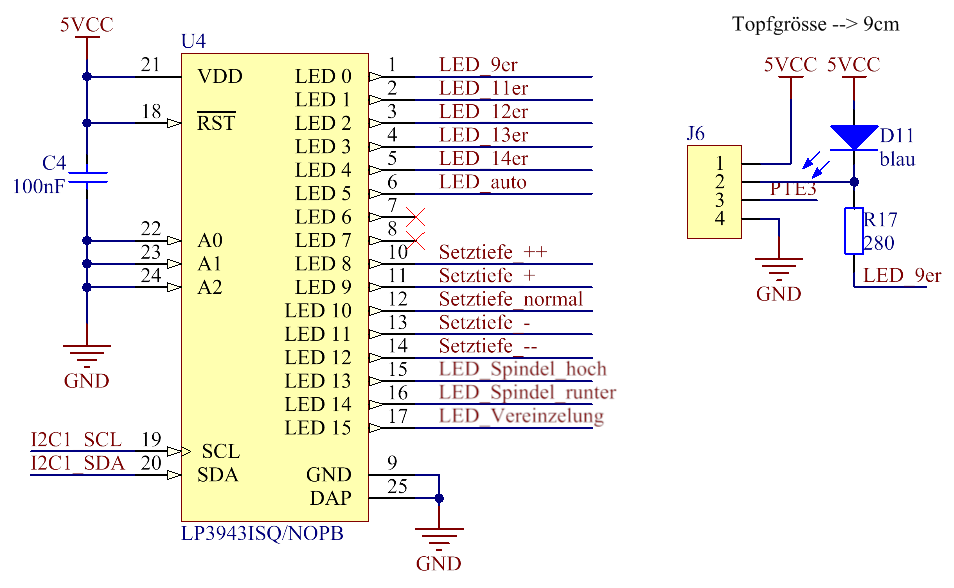
\includegraphics[width=0.7\textwidth]{Illustrationen/6-Umsetzung/Schema_Mainboard_LP39431.png}
	\caption{Schema Mainboard PCB, LED Treiber}
	\label{fig:Mainboard_LED_Driver_LP3943}
\end{figure}

Links ist der LED Treiber LP3943 zu sehen. Alle LEDs für das HMI sind daran angeschlossen. Über die Adressleitungen A0... A2 können die letzten 3 Bit der I$^{2}$C Adresse des Treibers bestimmt werden. In dieser Anwendung sind diese Digital Eingänge alle mit GND potential verbunden und somit auf logisch "0" konfiguriert. Auf der rechten Seite der Abbildung ist der Stecker J6 für einen Taster mit LED-Ring abgebildet. Alle HMI Taster mit LED-Ring werden jeweils über einen eigenen 4Pin Molex MicroFit Stecker verdrahtet (siehe Abb. \ref{fig:Mainboard_HMI_Layout}). Dabei wird der LED-Ring des Taster an Pin 1 und 2, der NO Kontakt an Pin 3 und der GND Kontakt an Pin 4 des Steckers angeschlossen.

\begin{figure}[H]
	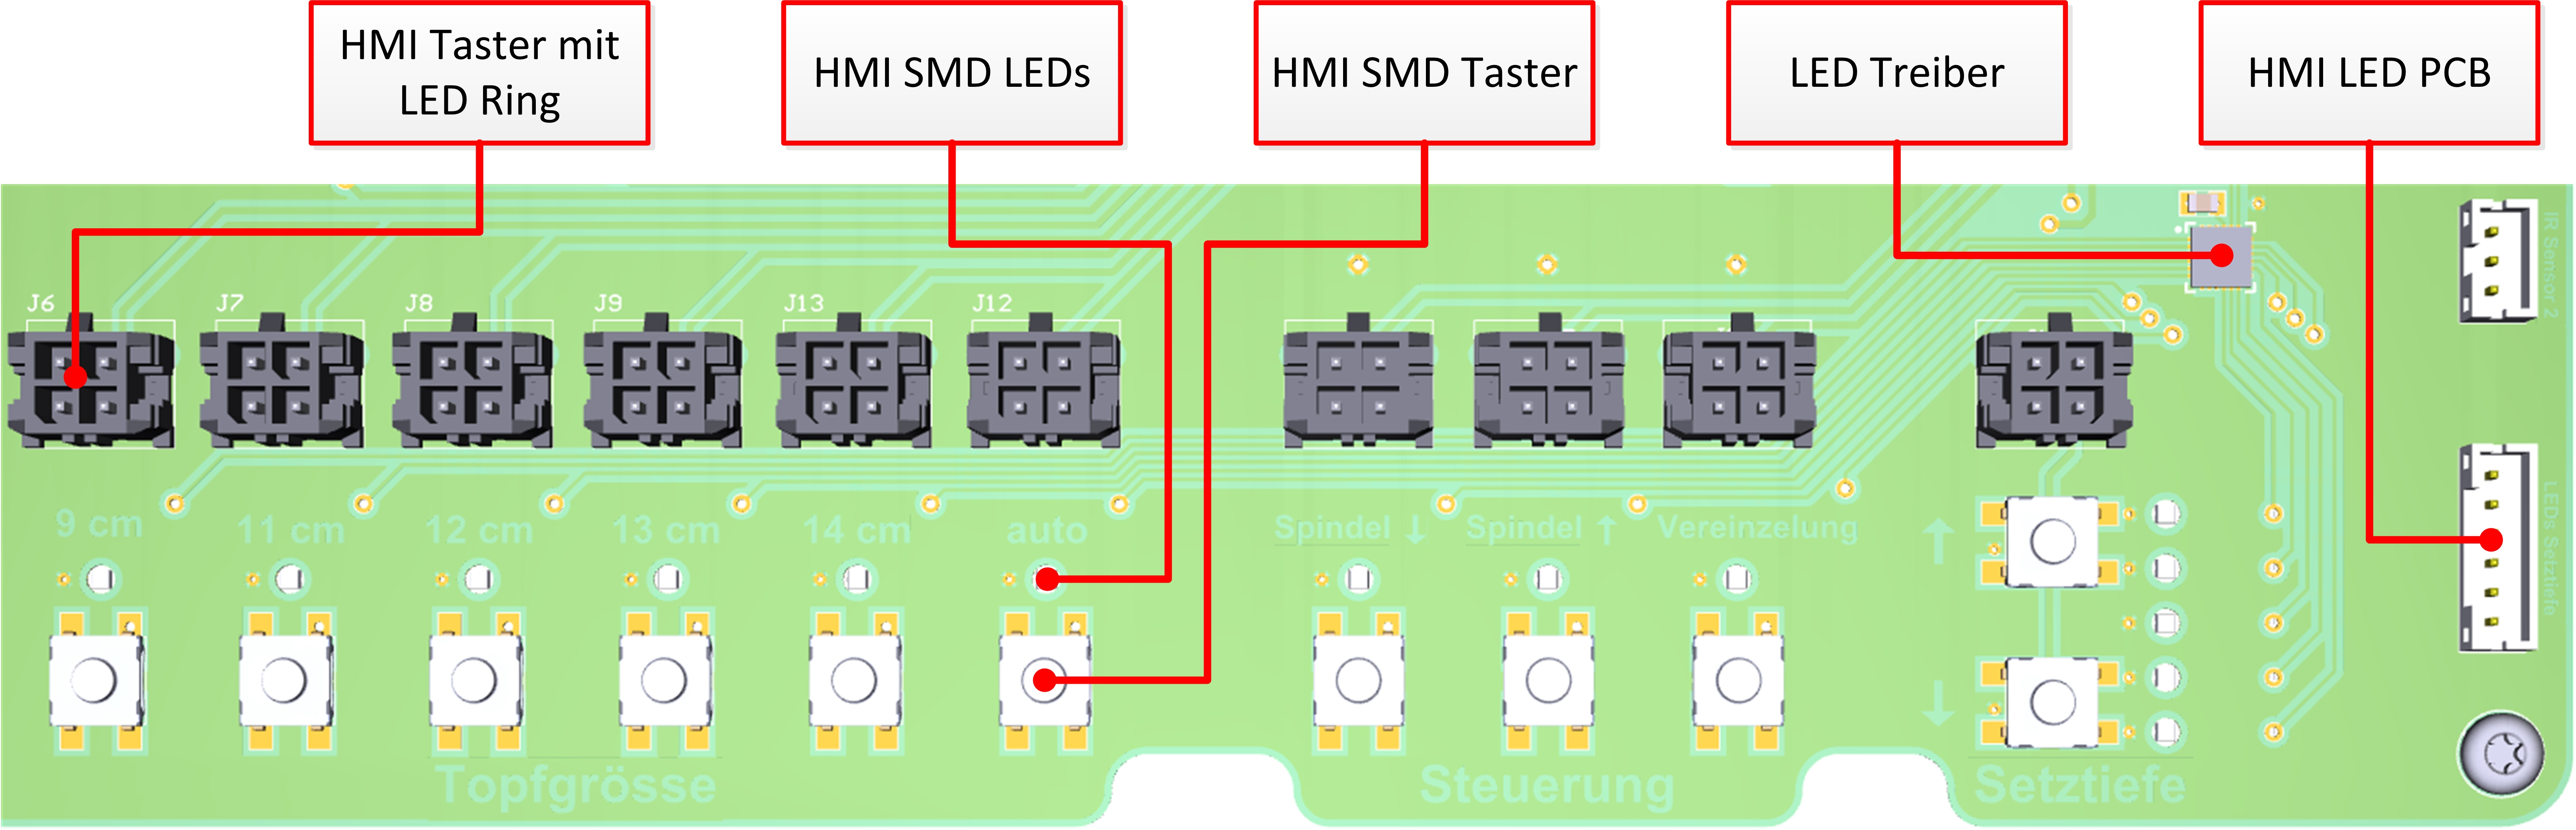
\includegraphics[width=1\textwidth]{Illustrationen/6-Umsetzung/HMI_Layout.jpg}
	\caption{Mainboard PCB, Onboard HMI}
	\label{fig:Mainboard_HMI_Layout}
\end{figure}

 Um die Software in Betrieb zu nehmen und zu testen, ohne das die Drucktaster verkabelt werden müssen, sind auf dem Mainboard bereits alle LEDs und Taster des HMI als SMD Bauteile bestückt. Alle LEDs auf dem Mainboard PCB sind $"$rear mounted$"$ LEDs. Diese werden auf dem Bottom Layer bestückt und leuchten durch eine Bohrung im PCB in Top Richtung. Durch diese Bauform bleibt mehr Platz auf dem Top Layer für Beschriftungen.




